%
% 3b21.tex
%
% 2018 Jonas Gründler, Hochschule Rapperswi
% 
% adaptiert von boxmodell.tex, 2018, Prof Dr Andreas Müller, Hochschule Rapperswil
%
\documentclass[tikz]{standalone}
\usepackage{times}
\usepackage{amsmath}
\usepackage{txfonts}
\usepackage[utf8]{inputenc}
\usepackage{graphics}
\usetikzlibrary{arrows,intersections}
\begin{document}
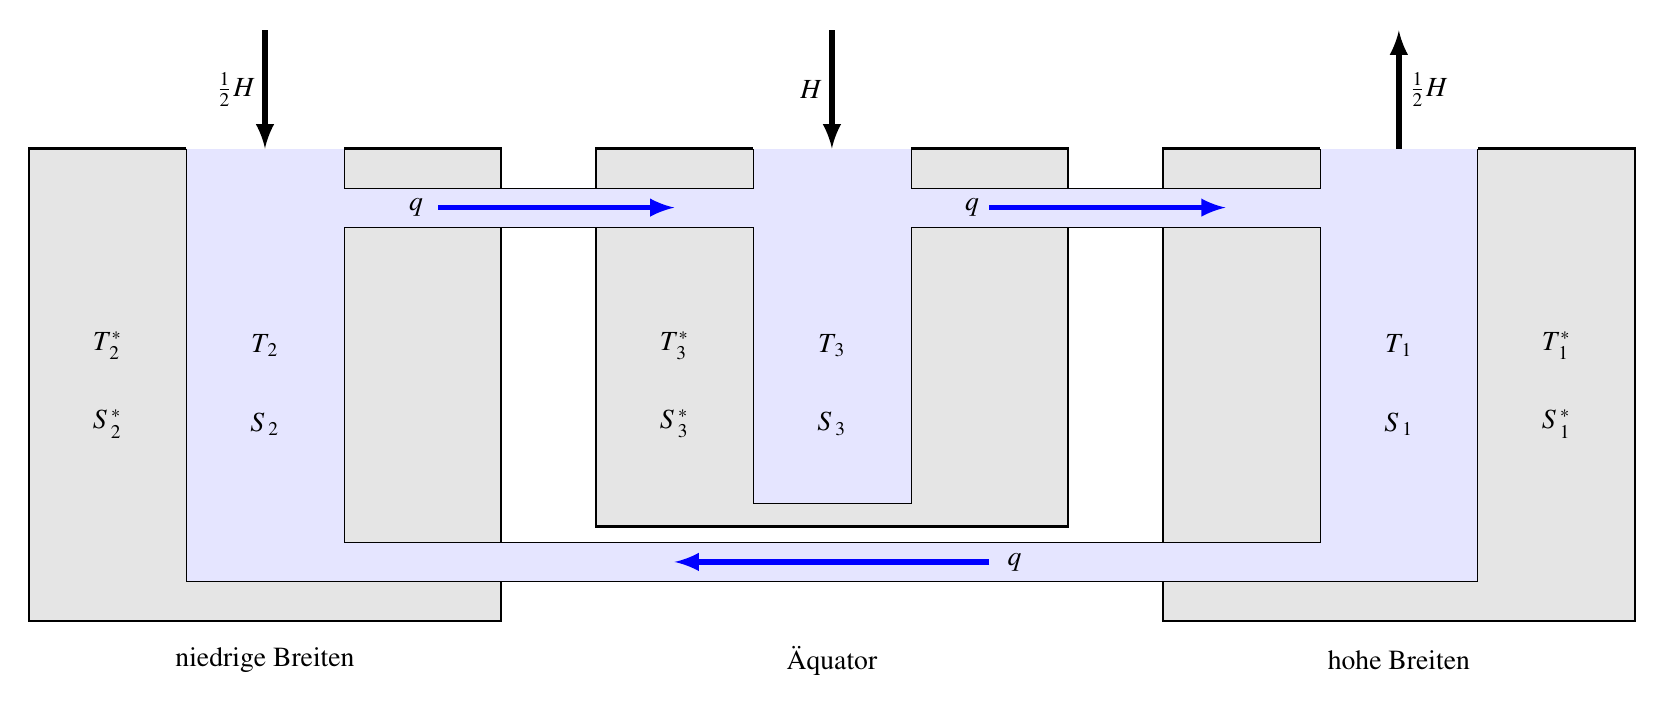
\begin{tikzpicture}[thick, >= latex, scale=1]

\def\gebietpole{
\fill[color=gray!20] (-3,-3)--(3,-3)--(3,3)--(-3,3)--cycle;
\draw (-3,-3)--(3,-3)--(3,3)--(-3,3)--cycle;
\fill[color=white] (-1,-2.5)--(1,-2.5)--(1,3.1)--(-1,3.1)--cycle;
\fill[color=blue!10] (-1,-2.5)--(1,-2.5)--(1,3.0)--(-1,3.0)--cycle;
}

\def\gebietaequator{
\fill[color=gray!20] (-3,-1.8)--(3,-1.8)--(3,3)--(-3,3)--cycle;
\draw (-3,-1.8)--(3,-1.8)--(3,3)--(-3,3)--cycle;
\fill[color=white] (-1,-1.5)--(1,-1.5)--(1,3.1)--(-1,3.1)--cycle;
\fill[color=blue!10] (-1,-1.5)--(1,-1.5)--(1,3.0)--(-1,3.0)--cycle;
}

\begin{scope}[xshift = -7.2cm]
\gebietpole
\node at (-2.0,0.5) {$T_2^*$};
\node at (-2.0,-0.5) {$S_2^*$};
\node at (0,0.5) {$T_2$};
\node at (0,-0.5) {$S_2$};
\node at (0,-3.5) {niedrige Breiten};
\draw[->,line width=2pt] (0,4.5)--(0,3);
\node at (0,3.75) [left] {$\frac{1}{2}H$};
\end{scope}

\begin{scope}
\gebietaequator
\node at (-2.0,0.5) {$T_3^*$};
\node at (-2.0,-0.5) {$S_3^*$};
\node at (0,0.5) {$T_3$};
\node at (0,-0.5) {$S_3$};
\node at (0,-3.5) {Äquator};
\draw[->,line width=2pt] (0,4.5)--(0,3);
\node at (0,3.75) [left] {$H$};
\end{scope}

\begin{scope}[xshift = 7.2cm]
\gebietpole
\node at (+2.0,0.5) {$T_1^*$};
\node at (+2.0,-0.5) {$S_1^*$};
\node at (0,0.5) {$T_1$};
\node at (0,-0.5) {$S_1$};
\node at (0,-3.5) {hohe Breiten};
\draw[<-,line width=2pt] (0,4.5)--(0,3);
\node at (0,3.75) [right] {$\frac{1}{2}H$};
\end{scope}

\fill[color=blue!10] (-7,-2.5)--(7,-2.5)--(7,-2)--(-7,-2)--cycle;
\fill[color=blue!10] (-7, 2.5)--(7, 2.5)--(7, 2)--(-7, 2)--cycle;


\draw[line width=0.1] (-8.2,3)--(-8.2,-2.5)--(8.2,-2.5)--(8.2,3);
\draw[line width=0.1] (-6.2,3)--(-6.2,2.5)--(-1,2.5)--(-1,3);
\draw[line width=0.1] (1,3)--(1,2.5)--(6.2,2.5)--(6.2,3);
\draw[line width=0.1] (-6.2,2)--(-6.2,-2)--(6.2,-2)--(6.2,2)--(1,2)--(1,-1.5)--(-1,-1.5)--(-1,2)--cycle;



\draw[->,line width=2pt,color=blue] (-5,2.25)--(-2,2.25);
\draw[->,line width=2pt,color=blue] (2,-2.25)--(-2,-2.25);

\draw[->,line width=2pt,color=blue] (2,2.25)--(5,2.25);
%\draw[->,line width=2pt,color=green] (5,-2.25)--(2,-2.25);

\node at (-5.5,2.25) [right] {$q$};
\node at (2,2.25) [left] {$q$};

\node at (2.1,-2.25) [right] {$q$};



\end{tikzpicture}
\end{document}

